\section{Basics of a Ch Mindstorms NXT Program}
To successfully control the Mindstorm NXT using Ch, it is 
important to practice good coding habits. The format of the Ch 
Mindstorm code is very similar to how a normal C code would be 
written, with the inclusion of some Ch specific functions and 
header files that are used to connect and control the NXT. The 
basic structure of a Ch NXT robot program is shown in the flow 
diagram in Figure \ref{fig_NXT_pstruc} below.\\
%%%%% START OF FIGURE %%%%%
\begin{figure}[h!]
  \begin{center}
    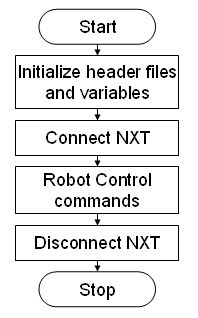
\includegraphics[height=3in]{figure/mindstorm/NXT_pstruc.png}
    \caption{Flow Diagram of a basic NXT program\label{fig_NXT_pstruc}}
  \end{center}
\end{figure}
%%%%% END OF FIGURE %%%%%
\subsection{Initialization}
In the beginning of a Ch Mindstorms NXT program or any C program,
you must include proper header files to run the program properly.
Without proper header files, the program will not have the 
specific libraries or source codes to run the program. Essential 
header files for the NXT includes:
\begin{verbatim}
    #include <conio.h>
    #include <nxt.h>
    #include <unistd.h>
\end{verbatim}
\noindent
The \verb+conio.h+ is an important header file that include the 
bluetooth connection functions that is required to establish 
connection between your PC and your NXT. This header also include
the \_kbhit() function, which is used to detect for hit "anykey" 
on keyboard if you want to pause your program. The \verb+nxt.h+ 
is the essential header file for Ch NXT function and variables.  
The \verb+unistd.h+ header is needed when using the 
\verb+delay()+ function, which is used when delays must be placed
into a program.

\subsection{Connect the NXT and Checking Connection Status}
The NXT status, sensor/encoder data, and input/output protocols 
are stored in a C++ class called \verb+ChNXT+. This class must be
created in every NXT program in order to connect. Therefore, in 
the beginning of your code, you must define a \verb+ChNXT+ class 
and use the \verb+connect()+ function to connect to the NXT. The 
\verb+connect()+ function will return a 0 if no connection is 
established, so you will have to terminate your program if no 
connection is established. An example of how to create the 
\verb+class+ and how to retrieve data are shown below:
\begin{verbatim}
    ChNXT nxt;

    /* Check status of NXT connection */
    if (!nxt.connect()){
        printf("Error: Cannot connect to Lego Mindstorm NXT.\n");
        exit(0);
    }
\end{verbatim}
The line \verb+ChNXT nxt;+ creates the class \verb+nxt+ that is 
used to store data and control the NXT robot. The function 
\verb+nxt.connect()+ called in the if statement is used to 
terminate the program in the event no connection is established. 
The \verb+printf()+ is included to print out an error message if 
\verb+nxt.connect+ fails. To end the program if connection fails,
the function \verb+exit()+ is used. The use of \verb+exit(0)+ is 
similar to the C function \verb+return(0)+, that can be used when
no \verb+main()+ function is present.

%%%%%%%%%%%%%% Advance Mindstorm Motor Control %%%%%%%%%%%%%
\subsection{Mindstorm Motor Control}
The following sections shows how to control the individual 
motors, and how the previously presented NXT vehicle actions can be done by controlling the individual motors.

%%%%%%%%%%%%%%%%%% Motor Control Functions %%%%%%%%%%%%%%%%%
\subsubsection{Motor Control Functions}
The function that is used to control the NXT motors is 
\verb+moveMotorContinuousNB()+. To use the function, you need the
motor port and the move direction. The speed of the motors are 
limited, and can only ranged from 0 to 100. For the direction, 1 
means positive direction and -1 means a negative direction. You 
will need to use the \verb+delay()+ function to leave the motors 
on for the desired amount of the time. For the setup of the NXT 
vehicle, forward motion can be achieved by turning the motors on 
to the same speed. For example:
\begin{verbatim}
    /* set speed */
    nxt.setMotorSpeeds(0, speed, speed);

    /* Move foward */
    nxt.moveMotorContinuousNB(NXT_MOTORB, 1);
    nxt.moveMotorContinuousNB(NXT_MOTORC, 1);

    /* Pause program for a while */
    delay(5);
\end{verbatim}
\noindent
This will move the NXT vehicle forward at the value the variable speed was set to. To get the 
NXT vehicle to move in reverse, the same code can be used by changing the sign on speed in the 
function \verb+setMotorSpeeds()+. The following shows the \verb+forwardBackward.ch+ rewritten to use 
the individual motor control.

%%%%%%%%%%  program 2 %%%%%%%%%%%%%
%%%%%%%%%%  program of forwardBackward.ch %%%%%%%%%%%%%
\verbatiminput{program/demo/forwardBackward.ch}
\begin{center}
Program 2: Ch program to move the NXT vehicle forward and backward.
\end{center}
%%%%%%%%%%%%%%%%%%%%%%%%% end %%%%%%%%%%%%%%%%%%%

%%%%%%%%%%%% Turning Using Single Motor Control %%%%%%%%%%%%
\subsection{Turning Using Single Motor Control}
Turning and rotation movements can also be achieved using the \verb+moveMotorContinuousNB()+ 
functions. As previously discussed, to turn our NXT vehicle, one motor must be rotating at a faster speed then the other, 
or the motors must be spinning in the opposite direction. For the following discussion, Figures \ref{fig_NXT_leftright} 
and \ref{fig_NXT_360LR} maybe useful.\\

\noindent
To turn the NXT vehicle left, the right wheel must be moving faster in forward direction then the 
left wheel.  The function \verb+vehicleTurnLeft()+ works by making the left wheel move at 0.7 of the 
speed that the right wheel is set to. To implement it with the single motor control functions, you 
would do the following:
\begin{verbatim}
    /* set speed */
    nxt.setMotorSpeeds(0, speed, 0.7*speed);

    /* Move foward-left */
    nxt.moveMotorContinuousNB(NXT_MOTORB, 1);
    nxt.moveMotorContinuousNB(NXT_MOTORC, 1);

    /* Pause program for a while */
    delay(5);
\end{verbatim}
\noindent
The value of 0.7 is somewhat arbitrary, and other constant values could be used to test the resulting
NXT vehicle response. The function \verb+vehicleRotateLeft()+ works similarly, instead setting the 
left wheel at the negative speed of the right wheel. An example is shown below:
\begin{verbatim}
    /* set speed */
    nxt.setMotorSpeeds(0, speed, speed);

    /* Rotate left in place */
    nxt.moveMotorContinuousNB(NXT_MOTORB, 1);
    nxt.moveMotorContinuousNB(NXT_MOTORC, -1);

    /* Pause program for a while */
    delay(5);
\end{verbatim}
\noindent
The \verb+vehicleTurnRight()+ and \verb+vehicleRotateRight()+ work similarly to \verb+vehicleTurnLeft()+
and \verb+vehicleRotateLeft()+, with only the commands to the motors reversed. Once you understand 
how the single motor commands work, more advance movements can be done, such as a move back and left 
motion.  The single motor commands can also be used to add a third motor attachment to the NXT 
vehicle, or used to control alternate robot designs that move or act differently.\\
\newline
\noindent
One alternative approach to implementing turning is to increase the speed of a wheel, instead of 
decreasing a wheel speed. For example, to implement a left turn, we could increase the speed of 
the right wheel by multiplying by a constant, such as 1.2.  The resulting code would look like:
\begin{verbatim}
    /* set speed */
    nxt.setMotorSpeeds(0, 1.2*speed, speed);
    /* Move foward-left */
    nxt.moveMotorContinuousNB(NXT_MOTORB, 1);
    nxt.moveMotorContinuousNB(NXT_MOTORC, 1);
    /* Pause program for a while */
    delay(5);
\end{verbatim}
\noindent
While this would work for slower motor speeds, a bug would occur if the NXT vehicle speed was 
set too high. Can you spot why? As previously discussed, the valid motor speeds for the NXT 
motors are between 0 to 100. If the speed variable is set to 100, the command to control 
the left motor (ROBOT\_MOTORC) will function correctly.  The right motor (ROBOT\_MOTORB) will recieve
a command telling it to set the motor speed to 1.2 x 100 = 120. This is an invalid motor 
command, and if you tried to run it on the NXT, it will cause the motor to reverse direction, 
making the NXT vehicle turn right instead of left. It is important to be watchful of these 
type of errors while writing code to control the NXT.\\
\newpage
% Controlling a NXT Vehicle %
\section{Controlling a NXT Vehicle}
%%%%% START OF FIGURE %%%%%
\begin{figure}[h!]
  \begin{center}
    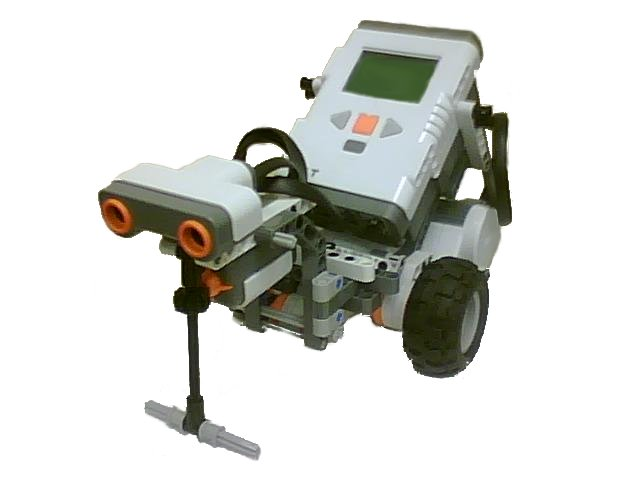
\includegraphics[height=3in]{figure/mindstorm/NXT_vehicle.png}
    \caption{NXT Vehicle\label{fig_NXT_vehicle}}
  \end{center}
\end{figure}
%%%%% END OF FIGURE %%%%%
\noindent
The NXT comes with three actuator output ports and the actuators available are the NXT motors. 
Normaly, you can only control the speed and direction of the connected motors. For a two wheeled NXT 
vehicle, there are two ways that the NXT vehicle can be controlled.  In addition to moving the NXT by
controlling the individual motors as shown in Figure \ref{fig_NXT_vehicle}, you can also use a set of
Ch mindstorm functions writen specificly to control an NXT vehicle. The diagram of the vehicle and 
the motor ports is shown in Figure \ref{fig_NXT_vehport}. When controlling the individual motors, you
would need to define the speed and direction of each motor.  The functions in the following examples 
require only a speed. In this section, we will show a basic Ch NXT program to move the robot forward.
Please make sure your NXT vehicle are configured according to to Figure \ref{fig_NXT_vehport} to run 
our demonstration programs.\\
%%%%% START OF FIGURE %%%%%
\begin{figure}[h]
  \begin{center}
    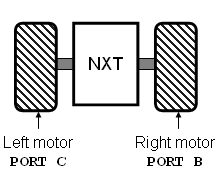
\includegraphics[height=2in]{figure/mindstorm/Vehicle.png}
    \caption{Motor configuration of the NXT Vehicle \label{fig_NXT_vehport}}
  \end{center}
\end{figure}
%%%%% END OF FIGURE %%%%%
%\subsection{Set the Motors' Speed}
%After creating a connection with the NXT, you can begin your program to control the NXT. Before make 
%motors move, the speed of three motors has to be set by using the function \verb+setMotorSpeed()+ to 
%setup a single motor or by using the function \verb+setMotorSpeeds()+ to setup speed for all three 
%motors. However, the speed of the motors are limited, and can only be set from 1 to 100. The following 
%shows how to setup speed for motors of Lego Mindstorms:

%\begin{verbatim}
%    /* setup speed for a single motor */
%    nxt.setMotorSpeed(NXT_MOTORA, 50);
%
%    /* setup speed for all motors */
%    nxt.setMotorSpeeds(20, 40, 40);
%\end{verbatim}

% END OF SET SPEED %
%\newline
%\\
\subsection{Moving the Robot Forward}
After setup speed for the motors, you can move the NXT vehicle forward by using the 
\verb+vehicleRollForward()+. After using the \verb+vehicleRollForward()+ function, you might want to 
allow some time for the motor to run by pausing the program for a few seconds. To pause the program 
from running for a few seconds, you can use the \verb+delay()+ function (each unit is 1 second, i.e. 
\verb+delay(1)+ = 1 second pause). Figure \ref{fig_NXT_forward} shows the NXT vehicle moving forward 
by actuating both wheels forward with the same speed, which is how the function \verb+vehicleRollForward()+ works. 
By default, the ports for the two wheels on the NXT are ROBOT\_MOTORB and ROBOT\_MOTORC.\\
%%%%% START OF FIGURE %%%%%
\begin{figure}[h]
  \begin{center}
    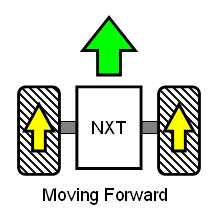
\includegraphics[height=2in]{figure/mindstorm/Vehicle_forward.png}
    \caption{Top-down view of NXT vehicle with two wheels\label{fig_NXT_forward}}
  \end{center}
\end{figure}
%%%%% END OF FIGURE %%%%%
\noindent
The following shows how the lego vehicle robot is moved forward in the \verb+vehicleRollForward.ch+ 
program:
\begin{verbatim}
    /* set speed */
    nxt.setSpeeds(0, 25, 25);
    /* Move foward */
    nxt.vehicleRollForward();
    /* Pause program for a while */
    delay(5);
\end{verbatim}

\subsection{Ending your program}
After you finish your program, you must end your program properly by stopping all the motors and 
disconnect the NXT from your computer. You can stop the motors using the \verb+stopAllMotors()+ function
, which stops all of the NXT motors. To disconnect the nxt, use the \verb+disconnect()+ function. For
example:
\begin{verbatim}
    /* Stop the motors */
    nxt.stopAllMotors();
    
    /* Disconnect NXT */
    nxt.disconnect();
\end{verbatim}

\subsection{forward.ch}
Now that the components of the program have been covered, \verb+vehicleRollForward.ch+ can now be run.
The code can be written using C or Ch syntax. For simplicity, the following code is presented as a Ch
program.

%%%%%%%%%%  program 1 %%%%%%%%%%%%%
%%%%%%%%%%  program of forward.ch %%%%%%%%%%%%%
\verbatiminput{program/demo/forward.ch}
\begin{center}
Program 1: Ch program to move the NXT vehicle forward.
\end{center}
%%%%%%%%%%%%%%%%%%%%%%%%% end %%%%%%%%%%%%%%%%%%%

\subsection{How to make your NXT move backward}
For a two wheeled NXT vehicle, you can make the vehicle move backward by using \verb+vehicleRollBackward()+. 
The function works like \verb+vehicleRollForward()+, moving the robot backwards. The function 
works by actuationg both wheels backward at the same speed, as shown in Figure \ref{fig_NXT_backward}.
%%%%% START OF FIGURE %%%%%
\begin{figure}[h]
  \begin{center}
    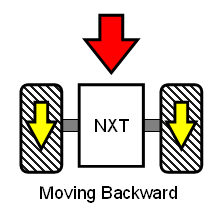
\includegraphics[height=2in]{figure/mindstorm/Vehicle_back.png}
    \caption{NXT vehicle moving backwards\label{fig_NXT_backward}}
  \end{center}
\end{figure}
%%%%% END OF FIGURE %%%%%
Using our new function, we can add the following code fragment to our first program to make the robot
move backwards. The code fragment is shown below:
\begin{verbatim}
    /* set speed */
    nxt.setMotorSpeeds(0, 25, 25);
    /* Move backward */
    nxt.vehicleRollBackward();
    delay(5);
\end{verbatim}
\noindent
The modified program is called: \verb+vehicleRollBackward.ch+.

\subsection{How to make your NXT move foward and left/right}
To make a two wheeled NXT vehicle to turn left or right while moving, one wheel must be moving 
faster than the other one.  For example, to move the NXT forward and turn left, both wheels will 
have to turn at a positive direction, and the right wheel must run faster than the left wheel. 
Figure \ref{fig_NXT_leftright} shows the NXT vehicle moving forward and left or right by actuating
both wheels forward with different speed.\\

%%%%% START OF FIGURE %%%%%
\begin{figure}[h]
  \begin{center}
    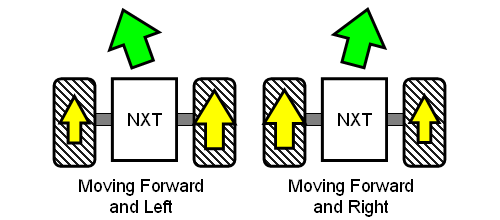
\includegraphics[height=2in]{figure/mindstorm/Vehicle_LR.png}
    \caption{NXT vehicle moving forward and left/right \label{fig_NXT_leftright}}
  \end{center}
\end{figure}
%%%%% END OF FIGURE %%%%%

\noindent
To make the NXT move forward and left/right, we can use the functions \verb+vehicleTurnLeft()+ 
and \verb+vehicleTurnRight()+. Like the previous NXT functions, a speed must be specified before 
using the function.  An example is shown below:
\begin{verbatim}
    /* set speed */
    nxt.setMotorSpeeds(0, 100, 70);
    /* Turn Left */ 
    nxt.vehicleTurnLeft();
    delay(5);
    
    //or
    
    /* set speed */
    nxt.setMotorSpeeds(0, 70, 100);
    /* Turn Right */
    nxt.vehicleTurnRight();
    delay(5);
\end{verbatim}
The modified programs are called: \verb+vehicleTurnLeft.ch+ and \verb+vehicleTurnRight.ch+.

\subsection{How to make your NXT turn in place left/right}

To make your NXT vehicle turn or rotate in place, the NXT vehicle wheels must be spun in the opposite
direction at the same speed. For example, to rotate the NXT vehicle to the left, the right wheel must
be spun forward, while the left wheel spins at the same speed in reverse. Figure \ref{fig_NXT_360LR} 
shown below shows the NXT vehicle turning in place left or right by actuating the wheels in opposite 
direction.
%%%%% START OF FIGURE %%%%%
\begin{figure}[h]
  \begin{center}
    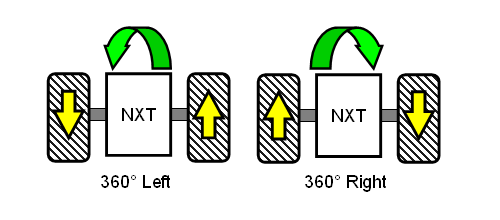
\includegraphics[height=2in]{figure/mindstorm/Vehicle_360LR.png}
    \caption{NXT vehicle turning 360 degrees \label{fig_NXT_360LR}}
  \end{center}
\end{figure}
%%%%% END OF FIGURE %%%%%
\noindent
To make the NXT rotate in place, we can use the functions \verb+vehicleRotateLeft()+ 
and \verb+vehicleRotateRight()+.  An example of how to use the functions are shown below:
\begin{verbatim}
    /* set speed */
    nxt.setMotorSpeeds(0, 50, 50);
    /* rotate left */
    nxt.vehicleRotateLeft();
    delay(5);
    
    // or
    
    /* set speed */
    nxt.setMotorSpeeds(0, 50, 50);
    /* rotate right */
    nxt.vehicleRotateRight();
    delay(5);
\end{verbatim}
\noindent
An example program is called: \verb+vehicleRotate.ch+.


\subsubsection{Manual Real Time Control Program}
Manual real time control program allows you to control your NXT vehicle with your keyboard like a 
remote control. For a manual control program, a user interface is usually used to display all the 
possible option that a user can input into the program. The user interface allow the user to know how
to control the NXT's motion. The NXT vehicle RTC program prints out a user interface for the user to 
use while executing the program. Figure \ref{fig_NXT_GUI} is the user interface of the NXT vehicle 
RTC program.\\
%%%%% START OF FIGURE %%%%%
\begin{figure}[h]
  \begin{center}
    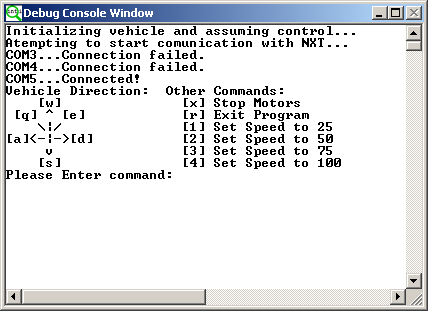
\includegraphics[height=3in]{figure/mindstorm/RTC_GUI.png}
    \caption{NXT vehicle RTC User Interface \label{fig_NXT_GUI}}
  \end{center}
\end{figure}
%%%%% END OF FIGURE %%%%%
\\
In Figure \ref{fig_NXT_GUI}, the user interface of the NXT vehicle RTC program display all the 
possible key that the user can use. In addition, the user interface also indicate the functionality 
of the key that is being pressed. When a specific key is pressed during the execution of the NXT 
vehicle RTC program, the program uses a \verb+switch()+ statement to performs a fragment of code that
send commands to the NXT.
For example:\\
\begin{itemize}
\item The key \verb+"w"+ is to control the NXT to move forward.
\item The key \verb+"s"+ is to control the NXT to move backward.
\item The key \verb+"a"+ is to control the NXT to turn left.
\item The key \verb+"d"+ is to control the NXT to turn right.
\item The key \verb+"x"+ is to stop the NXT motors.
\item The key \verb+"1"+ is to set the NXT motor speed to 25.
\item The key \verb+"r"+ is to exit the manual RTC program.
\end{itemize}

\noindent
In the robot control code block, a while loop is implemented to allow the user to control the NXT
continuously until the program is terminated. Within the while loop, the program grabs the user's 
input and decide what to do with it using the \verb+switch+ and \verb+case+ statements.
The whole NXT vehicle RTC program is shown in Program 2. Please make sure your NXT vehicle are 
configured according to to Figure \ref{fig_NXT_vehport} to run Program 2. In the rest of this 
section, we are going to explain the whole program in detail.

%%%%% Program 2 %%%%%
\verbatiminput{program/mindstorm/vehicle_rtc.ch}
\begin{center}
Program 2: Manual Real Time Control Program for NXT vehicle.
\end{center}
%%%%% End of Program 2 %%%%%%

\subsubsection*{Header files}
Similar to any C program, you will have to include necessary header files, which is described in the 
first four lines.
    
\begin{verbatim}
    #include <conio.h>
    #include <stdio.h>
    #include <nxt.h>
    #include <unistd.h>
\end{verbatim}

\begin{itemize}
\item The header \verb+conio.h+ provides a function for the program to detect a key press for the
\verb+-press a key-+ command.
\item The header \verb+stdio.h+ provides input and output function for the program. These input and 
output function allows the program to display output for the user or ask for the user input.
\item The header \verb+nxt.h+ provides the program with general functions of the Ch Mindstorm 
Control Package.
\end{itemize}

\subsubsection*{Declaring variables}
After including the headers, the C program will start the \verb+main()+ program.
Like any C programs, you must declare variables before you can use them.
On the top few lines of the \verb+main()+ program, variables are declared.
\begin{verbatim}
    ChNXT nxt;
    int speed = 25,	//speed of the motors. (default to 25)
        quit = 0,	//used by quit case to exit the loop
        status1,	//used to check for errors
        status2;	//used to check for errors
    char key = 'x',	//stores the input from the user
        movemode = 'x';//stores the last movement command
\end{verbatim}

\begin{itemize}
\item The \verb+ChNXT+ class stores the connection status, sensor data, and motor counter data of the
    NXT. Also, the class includes the functions for controling the NXT.
\item The integer variable \verb+speed+ stores the speed of the motor.
\item The integer variable \verb+quit+ is used to check if the user wants to quit the program.
\item The integer variable \verb+status1+ and \verb+status2+ are used to check the sensor connection.
\item The character variable \verb+key+ stores the input from the user.
\item The character variable \verb+movemode+ stores the last command that the user used.
\end{itemize}

\subsubsection*{Checking connection}
After declaring variables, the connection of the NXT needs to be checked.
In the next 7 lines of the program, the program checks for the connection of the NXT to the computer.
If the NXT connection fails, the program will quit.
\begin{verbatim}
    /* Connect to NXT */
    printf("Initializing vehicle and assuming control...");
    if (!nxt.connect()){
        printf("\nPress any key to exit.\n");
        while (!_kbhit()); //wait for keypress
        exit(0);
    }
\end{verbatim}

\subsubsection*{User interface}
Before the beginning of the real time control, the user must be able to know the function of the key 
they are pressing. To do this, the program print out a user interface for the user to read. 
In segment of the Program 4 shown below, the NXT vehicle RTC program used \verb+printf()+ command is 
used to display the user interface for the user to read.
\begin{verbatim}
    /* GUI display */
    printf("Vehicle Direction:  Other Commands:");
    printf("\n    [w]               [x] Stop Motors");
    printf("\n [q] ^ [e]            [r] Exit Program");
    printf("\n    \|/               [1] Set Speed to 25");
    printf("\n[a]<-|->[d]           [2] Set Speed to 50");
    printf("\n     v                [3] Set Speed to 75");
    printf("\n    [s]               [4] Set Speed to 100\n");
    printf("Please Enter command:");
\end{verbatim}

\subsubsection*{Real time control}
After completing the initiation of the code, which include adding header files, declaring variables,
checking connection, and displaying the user interface, the real time control of the NXT begins with 
the robot control code block. In the robot control code block, a while loop is implemented to allow 
the user to control the NXT continuously until the program is terminated. Within the while loop, the 
program grabs an input from the user, and then decide what to do with the input using the 
\verb+switch()+ and \verb+case+ statement. A basic flow diagram of the control loop for the NXT 
vehicle RTC program is shown in Figure \ref{fig_RTC_controlloop} below.\\
    
\begin{figure}[h]
  \begin{center}
    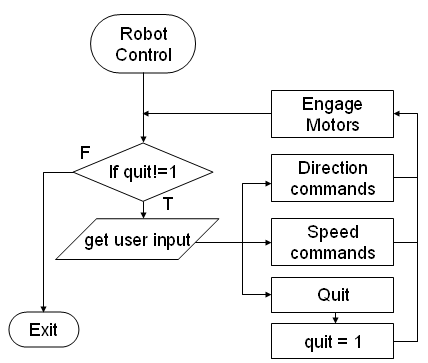
\includegraphics[height=2.4in]{figure/mindstorm/RTC_controlloop.png}
    \caption{NXT vehicle RTC Control Loop Flow Diagram \label{fig_RTC_controlloop}}
  \end{center}
\end{figure}

\noindent
The program fragment shown below shows the beginning and the end of the while loop for Program 4:
\begin{verbatim}
    while (quit != 1 ) {
        key = _getch();
        switch (key){
        
        ...
        
        }
    }
\end{verbatim}
\noindent
When the program reaches this stage, the real time control begins. The while loop allows the program 
to keep asking the user's input until the \verb+'r'+ key is pressed. When the \verb+'r'+ key is 
pressed, the program will set \verb+quit+ variable is set to 1, which allows the program to exit 
out of the while loop.\\ \\
\noindent
For first line of the while loop, the program use the \verb+_getch()+ command to obtain a user
input and store the user input to the variable \verb+key+. After obtaining the user's input in a 
variable, the program use a \verb+switch()+ function to check which key was pressed. Depending on 
what key was pressed, the program will run a fragment of code that sends commands to the NXT.

\subsubsection*{Directional commands}
The movements are controlled using the 'w', 's', 'a', and 'd' format. In Figure \ref{fig_NXT_GUI}, 
the user interface used arrows to indicate the movement direction and associate each direction with 
a specific key. The available buttons for movements are 'w', 's', 'a', 'd', 'q', 'e', and 'x'.
\\ \\
%%% case 'w' %%%
\noindent
When the key 'w' has been pressed, the \verb+switch()+ function will run the codes for the case 'w'.
The program fragment for case 'w' is shown below:
\begin{verbatim} 
    case 'w': //up
        nxt.moveMotorContinuousNB(NXT_MOTORB, 1);
        nxt.moveMotorContinuousNB(NXT_MOTORC, 1);
        movemode = 'w';
        break;
\end{verbatim}
In case 'w', the program will run the motor in \verb+NXT_MOTORB+ and \verb+NXT_MOTORC+ forward at
the velocity \verb+speed+, and then set the motor to run idle mode. Next, 'w' key is stored in the 
variable \verb+movemode+, which will be used to indicate the current mode for NXT vehicle. Basically,
the case 'w' will move the NXT vehicle forward with velocity \verb+speed+.
\\ \\
%%% case 's' %%%
\noindent
When the key 's' has been pressed, the \verb+switch()+ function will run the codes for the case 's'.
The program fragment for case 's' is shown below:
\begin{verbatim} 
    case 's': //down
        nxt.moveMotorContinuousNB(NXT_MOTORB, -1);
        nxt.moveMotorContinuousNB(NXT_MOTORC, -1);
        movemode = 's';
        break;
\end{verbatim}
In case 's', the program will run the motor in \verb+NXT_MOTORB+ and \verb+NXT_MOTORC+ backward 
at the velocity \verb+speed+, and then set the motor to run idle mode. Next, 's' key is stored in the
variable \verb+movemode+, which will be used to indicate the current mode for NXT vehicle. Basically,
the case 's' will move the NXT vehicle backward with velocity \verb+speed+.
\\ \\
%%% case 'a' %%%
\noindent 
When the key 'a' has been pressed, the \verb+switch()+ function will run the codes for the case 'a'.
The program fragment for case 'a' is shown below:
\begin{verbatim} 
    case 'a': //left
        nxt.moveMotorContinuousNB(NXT_MOTORB, 1);
        nxt.moveMotorContinuousNB(NXT_MOTORC, -1);
        movemode = 'a';
\end{verbatim}
In case 'a', the program will actuate motor in \verb+NXT_MOTORB+ forward at velocity \verb+speed+ 
and actuate motor in \verb+NXT_MOTORC+ backward at velocity \verb+speed+. Next, 'a' key is stored in the variable \verb+movemode+, which will be used to 
indicate the current mode for NXT vehicle.
\\ \\
%%% case 'd' %%%
\noindent
When the key 'd' has been pressed, the \verb+switch()+ function will run the codes for the case 'd'.
The program fragment for case 'd' is shown below:
\begin{verbatim} 
    case 'd': //right
        nxt.moveMotorContinuousNB(NXT_MOTORB, -1);
        nxt.moveMotorContinuousNB(NXT_MOTORC, 1);
        movemode = 'd';
        break;
\end{verbatim}
In case 'd', the program will actuate motor in \verb+NXT_MOTORB+ backward at velocity \verb+speed+ 
and actuate motor in \verb+NXT_MOTORC+ forward at velocity \verb+speed+. Next, 'd' key is stored in
the variable \verb+movemode+, which will be used to indicate the current mode for NXT vehicle.
\\ \\
%%% case 'q' %%%    
\noindent
When the key 'q' has been pressed, the \verb+switch()+ function will run the codes for the case 'q'.
The program fragment for case 'q' is shown below:
\begin{verbatim} 
    case 'q': //forward-left
        nxt.setMotorSpeeds(0, speed, 0.7*speed);
        nxt.moveMotorContinuousNB(NXT_MOTORB, 1);
        nxt.moveMotorContinuousNB(NXT_MOTORC, -1);
        movemode = 'q';
        break;
\end{verbatim}
In case 'q', the program will actuate motor in \verb+NXT_MOTORB+ forward at velocity \verb+speed+ 
and actuate motor in \verb+NXT_MOTORC+ forward at velocity 0.7*\verb+speed+. Next, 'q' key is 
stored in the variable \verb+movemode+, which will be used to indicate the current mode for NXT 
vehicle.
\\ \\
%%% case 'e' %%%
\noindent 
When the key 'e' has been pressed, the \verb+switch()+ function will run the codes for the case 'e'.
The program fragment for case 'e' is shown below:
\begin{verbatim} 
    case 'e': //forward-right
        nxt.setMotorSpeeds(0, 0.7*speed, speed);
        nxt.moveMotorContinuousNB(NXT_MOTORB, -1);
        nxt.moveMotorContinuousNB(NXT_MOTORC, 1);
        movemode = 'e';
        break;
\end{verbatim}
In case 'e', the program will actuate motor in \verb+NXT_MOTORB+ forward at velocity 
0.7*\verb+speed+ and actuate motor in \verb+NXT_MOTORC+ forward at velocity \verb+speed+. Next, 'e'
key is stored in the variable \verb+movemode+, which will be used to indicate the current mode for 
NXT vehicle.
\\ \\
%%% case 'x' %%%
\noindent
When the key 'x' has been pressed, the \verb+switch()+ function will run the codes for the case 'x'.
The program fragment for case 'x' is shown below:
\begin{verbatim} 
    case 'x': //stop
        nxt.stopOneMotor(NXT_MOTORB);
        nxt.stopOneMotor(NXT_MOTORC);
        movemode = 'x';
        break;
\end{verbatim}
In case 'x', the program will set the motor in \verb+NXT_MOTORB+ and \verb+NXT_MOTORC+ to zero 
velocity, and then set the motor to off idle mode. Next, 'x' key is stored in the variable 
\verb+movemode+, which will be used to indicate the current mode for NXT vehicle.
Basically, the case 'x' stops the motor and keep it turned off until another key is pressed.

\subsubsection*{Speed control}
The speed of the motor is controlled by the number key '1', '2', '3', and '4'.
In Figure \ref{fig_NXT_GUI}, the user interface shows that each key has a specific speed.
For example, key '1' indicates 25 speed, and key '2' indicate 50 speed.
As shown below, each of the key has its fragment of code.

\begin{verbatim}
    case '1': //speed 25
        speed = 25;
        ungetch(movemode);
        break;
    case '2': //speed 50
        speed = 50;
        ungetch(movemode);
        break;
    case '3': //speed 75
        speed = 75;
        ungetch(movemode);
        break;
    case '4': //speed 100
        speed = 100;
        ungetch(movemode);
        break;
\end{verbatim}
\noindent
For each of the case, the fragment of code changes the variable \verb+speed+ and performs an \verb+ungetch()+ command.
The \verb+ungetch()+ command allows the program run the mode that it was previously saved in the variable \verb+movemode+
before the speed keys are pressed. Basically, the speed keys allow the program to change the speed of the NXT motor without 
changing the movement mode that it was in.

\subsubsection*{Functions for other keys}
As mentioned before, the while loop allows the program to keep asking the user's input until the variable
\verb+quit+ is set to 1. To quit the while loop, we must have a special case that sets the variable \verb+quit+ to 1.
When the key 'r' is pressed, the \verb+switch()+ function will perform a fragment of code for case 'r'.
The program fragment for case 'r' is shown below:
\begin{verbatim}
    case 'r': //quit
        printf("\nExiting program.\n");
        quit = 1;
        break;
\end{verbatim}
\noindent
When the \verb+'r'+ key is pressed, the program will print out the statement 'exiting program' and set \verb+quit+
variable is set to 1, which allows the program to exit out of the while loop.
\newline
For the keys that is not specified to any cases, a default case is used for the time when the user input a wrong key.
The program fragment for the default case is shown below:
\begin{verbatim}
    default:
        printf("\nInvalid Input!\n");
\end{verbatim}
\noindent
This fragment prints 'Invalid Input!' to the user to indicate the key they just pressed is an invalid input.

\subsubsection*{Disconnecting your NXT}
After the while loop, the NXT vehicle RTC program ends with the four lines shown below.
\begin{verbatim}
    nxt.disconnect();   //stop interfacing. This also stops the motors.
    printf("Press any key to exit.\n");
    while (!_kbhit()); //wait for key press
\end{verbatim}
\noindent
These lines of code stop the NXT motors, disconnect the NXT from the computer, ask for the user
to press a key, and terminate  the program.
%%%%%%%%%% end of NXT RTC %%%%%%%%%%
%%%%%%%%%%% End of Controlling NXT Vehicle %%%%%%%%%%

%%%%%%%%%%% Using NXT Sensors %%%%%%%%%%
\subsection{Using NXT Sensors}
Sensors converts a physical quantity and convert it to signals which can be read by the NXT or the computer. 
Sensors allows the communication between the outside environment to the NXT. The NXT is equipped with four 
sensor input ports and you can equip each port with a variety of different sensors. In this section, we are 
going to discuss about how to use the touch sensor and the ultrasonic sensor. In these discussion, two 
demonstration program will be presented. Please make sure your NXT vehicle are configured according to to 
Figure \ref{fig_NXT_sensport} to run these demonstration programs.
%%%%% START OF FIGURE %%%%%
\begin{figure}[h]
  \begin{center}
    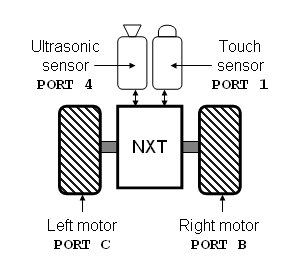
\includegraphics[height=2.4in]{figure/mindstorm/NXT_auto.png}
    \caption{Sensor/Motor configuration of the NXT Vehicle \label{fig_NXT_sensport}}
  \end{center}
\end{figure}
%%%%% END OF FIGURE %%%%%
\subsubsection{Using your touch sensor}
After you have connected your NXT to your PC, you will need to set up the sensor if you would like to include 
sensors in your NXT program. For example, if you want to add components like light sensor, ultrasonic sensor, 
and/or touch sensor, you will need to set up their connection using the \verb+setSensor()+ function. 
The \verb+setSensor()+ function will return 0 if no connection is established, so you can terminate the 
program if a sensor connection is not established. An example connection check for adding the Touch and 
Ulstrasonic sensors to the NXT vehicle is as follow:
\begin{verbatim}
    ChNXT nxt;

    /* Check status of NXT connection */
    if (!nxt.connect()){
        exit(0);
    }
    
    /* Setup sensors and check sensor connection */
    int status1=2, status2=2;

    /* Save status of SENSOR_PORT1, and SENSOR_PORT4 */
    status1=nxt.setSensor(SENSOR_PORT1,SENSOR_TYPE_TOUCH,BOOLEANMODE);
    status2=nxt.setSensor(SENSOR_PORT4,SENSOR_TYPE_ULTRASONIC,RAWMODE);
    
    /* Check connection status of SENSOR_PORT1 */
    if(status1==0) {
        exit(0);
    }
    
    /* Check connection status of SENSOR_PORT4 */
    if(status2==0) {
        exit(0);
    }
\end{verbatim}
As in previous examples, the nxt\_remote stucture, \verb+nxtr+, is created, and the initial connection 
to the NXT is made. The next step is to initialize the NXT sensor ports to the correct types and ensure 
the sensors are working correctly.  The int variables \verb+status1+ and \verb+status2+ are used to 
check the return value of the function \verb+setSensor()+.
//
A common application of touch sensors for a vehicle robot is for obstacle detection. In order to 
demonstrate the use of the touch sensor, consider the touch sensor demo in Program 3.

%%%%% Program 3 %%%%%
\verbatiminput{program/mindstorm/touchsensor.ch}
\begin{center}
Program 3: Ch NXT touch sensor demonstration program.
\end{center}
%%%%% End of Program 3 %%%%%%

\subsubsection*{Checking touch sensor connection}
Program 3 is similar to Program 1, the only changes is the addition of the use of the touch sensor. Program 3 
makes the NXT move forward until the touch sensor is triggered, after which it will back up and stop. One of 
the additions that is added in Program 3 is the initialization of the touch sensor. The fragment of the 
initialization of the touch sensor is shown below.
\begin{verbatim}
    /* Set sensor types */
    int status;
    status = nxt.setSensor(SENSOR_PORT1, SENSOR_TYPE_TOUCH, BOOLEANMODE);
    if (status == 0){
        exit(0);
    }
\end{verbatim}
In this fragment, the program use the \verb+setSensor()+ command to set the touch sensor to \verb+PORT 1+. 
The connection status between the NXT and the sensor is then returned in the variable called status. Next, the 
if statement check if the connection to the sensor is good. If the variable status is equal to 0, which means
 no sensor connection, the program will be exited and the rest of the codes will not be executed.
 
\subsubsection*{Using while loop}
A while loop is a common method that is used for sensor data gathering. For every iteration of the while loop, 
the program checks the data gathered by the touch sensor. After gathering the data, the program decide what to 
do with the data. A simple flow diagram of the while loop of the touch sensor demo program is shown in Figure 
\ref{fig_NXT_touchflow}\\

%%%%% START OF FIGURE %%%%%
\begin{figure}[h]
  \begin{center}
    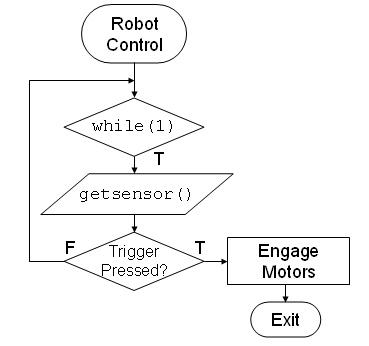
\includegraphics[height=2.4in]{figure/mindstorm/NXT_touchflow.png}
    \caption{Flow Diagram of the while loop in Program 3 \label{fig_NXT_touchflow}}
  \end{center}
\end{figure}
%%%%% END OF FIGURE %%%%%
\noindent
In Program 3, the while loop checks for the data of the touch sensor. If the touch sensor is triggered, 
the data of the touch sensor will be set to below 500. Then the program will move the NXT backward and 
disconnect the NXT. The while loop of the touch sensor demonstration program is described below:
\begin{verbatim}
    while(1){
        /* Get touch sensor data and save into a variable*/
        touchValue = nxt.getSensor(SENSOR_PORT1);
        /* If touch sensor is triggered */
        if (touchValue < 500){
            //Move backward
            nxt.setMotorSpeeds(0, 25, 25);
            nxt.vehicleRollBackward();
            delay(5);
            break;
        }
    }
\end{verbatim}
In this while loop, the program uses the \verb+getSensor()+ command to get the data from \verb+PORT 1+, 
which is the port for the touch sensor according to Figure \ref{fig_NXT_sensport}. Next, the program checks 
the touch sensor if it is pressed with the if statement. If the touch sensor has been triggered, the codes 
in the if statement will run. The codes inside the if statement is the same command for moving the NXT 
backward. After moving the NXT backward, the command break allows the program to exit out of the while loop.
 This while loop will never exit until the touch sensor is triggered and the break command is used.

\subsubsection{Using your ultrasonic sensor}
In order to demonstrate the use of the ultrasonic sensor, consider the ultrasonic sensor demo in Program 4.
NOTE: If your robot gets stuck, put your hands in front of the ultrasonic sensor to quit the loop.

%%%%% Program 4 %%%%%
\verbatiminput{program/mindstorm/ultrasonicsensor.ch}
\begin{center}
Program 4: Ch NXT ultrasonic sensor demonstration program.
\end{center}
%%%%% End of Program 4 %%%%%%

\subsubsection*{Checking touch sensor connection}
Like Program 3, Program 4 is meant to be a brief demonstration of one method of using an ultrasonic sensor 
with a vehicle NXT.
Similar to the initialization of the touch sensor, the initialization of the ultrasonic sensor is shown below:

\begin{verbatim}
    /* Set sensor types */
    int status;
    status = nxt.setSensor(SENSOR_PORT4, SENSOR_TYPE_ULTRASONIC, RAWMODE);
    if (status == 0){
        exit(0);
    }
\end{verbatim}
In this program fragment, the \verb+setSensor()+ command sets the ultrasonic sensor to \verb+PORT 4+.
Next, it checks the return value of the sensor connection status.
The program will quit if the return value is 0, meaning there is no connection between the sensor and the NXT.

\subsubsection*{Contents in the while loop}
In Program 4, the while loop uses the ultrasonic sensor to detect distances between the NXT and the obstacles in 
front of the NXT. The ultrasonic sensor will detect distances and the program code reacts to the data by slowing 
down or speeding up. The flow diagram of the while loop of Program 4 is shown in Figure \ref{fig_NXT_ultraflow}.
%%%%% START OF FIGURE %%%%%
\begin{figure}[h]
  \begin{center}
    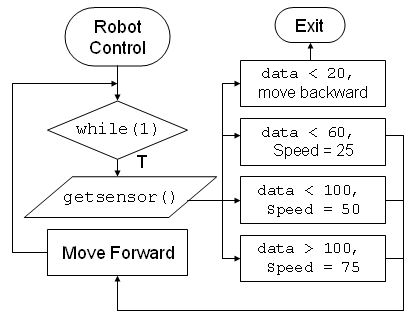
\includegraphics[height=2.4in]{figure/mindstorm/NXT_ultraflow.png}
    \caption{Flow Diagram of the while loop in Program 3 \label{fig_NXT_ultraflow}}
  \end{center}
\end{figure}
%%%%% END OF FIGURE %%%%%

The while loop code block for Program 4 is shown below:
\begin{verbatim}
    //Commands:
    while(1){
        /* Get ultrasonic sensor data */
        ultrasoniceValue = nxt.getSensor(SENSOR_PORT4);
        /* If obstacle is really close */
        if (ultrasonicValue < 20){
            speed = 25;
            /* Move backward */
            nxt.setMotorSpeeds(0, speed, speed);
            nxt.vehicleRollBackward();
            delay(3);
            /* Quit the while loop */
            break;
        }
        /* Else if the obstacle is close */
        else if(ultrasonicValue < 60){
            speed = 25;
        }
        /* Else if the obstacle is not close */
        else if(ultrasonicValue < 100){
            speed = 50;
        }
        /* Else if there is no obstacle in sight */
        else if(ultrasonicValue < 200){
            speed = 75;
        }
        //Sensor value larger than 200
        else{
            speed = 75;
        }
        /* Move forward (constantly) */
        nxt.setMotorSpeeds(0, speed, speed);
        nxt.vehicleRollForward();
    }
\end{verbatim}
\noindent
Similar to Program 3, the while loop in Program 4 also gathers the sensor data using the
    \verb+getSensor()+ command to gather data from the ultrasonic sensor in \verb+PORT 4+.
Next, the if-else statement block determine what to do depending on the distance data from ultrasonic sensor.
\begin{itemize}
\item If the sensor value is below 20, which means the vehicle is very close to an obstacle, the program tells the
    vehicle to reverse, and then break out of the while loop.
\item If the sensor value is above 20 and below 60, which means the vehicle is close to an obstacle, the
    program set the speed variable to 25.
\item If the sensor value is above 60 and below 100, which means the vehicle is not close to an obstacle, the
    program set the speed variable to 50.
\item If the sensor value is above 100 and below 200, which means there is nothing in front of the vehicle,
    the program set the speed variable to 75.
\item If the sensor value is other value that is not mentioned above, the program set the speed variable to 75.
\end{itemize}
After the if-else statement block, the program sets the robot to move forward with velocity set at the speed variable.
Then the program returns back to the beginning of the while loop, which is to gather data from the sensor again.

%%%%%%%%%% NXT auto %%%%%%%%%%
\subsubsection{Autonomous Control Program}
In the previous sections, we thoroughly covered the manual real time control program, which allows you to 
remote control your NXT vehicle with your keyboard.
In this section, we will talk about the autonomous control program for the NXT vehicle.
In an autonomous control program, the robot, which is the NXT, must be able to move around by itself without
human commands or interventions. In order to achieve such task, the NXT must be able to detect obstacles using 
its sensors and steer away from the obstacle using its actuators.
A typical autonomous control scheme is to sense, plan, and act, which is shown in Figure \ref{fig_NXT_SPA}.
%%%%% START OF FIGURE %%%%%
\begin{figure}[h]
  \begin{center}
    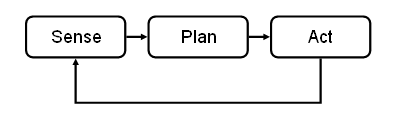
\includegraphics[height=1in]{figure/mindstorm/Senseplanact.png}
    \caption{Sense Plan Act Diagram \label{fig_NXT_SPA}}
  \end{center}
\end{figure}
%%%%% END OF FIGURE %%%%%
\begin{itemize}
\item Sense is to gather data from the robot's surrounding.
\item Plan is to plan the interaction between the robot and its surrounding using gathered data.
\item Act is to act with robot's surrounding.
\end{itemize}
The main difference between the manual RTC program and the autonomous program is the content inside the while loop.
In the manual RTC program, the codes inside the while loop scan for user's input and the robot acts on the input that
the user provided. In the autonomous program, the codes inside the while loop perform the sense-plan-act cycle similarly 
to the diagram shown in Figure \ref{fig_NXT_SPA}.
Every cycle, the information is gathered from the sensor and send back to the computer.
The computer will decide what to do depending on the sensor data.
The autonomous control program for the NXT vehicle is described in Program 5.
%%%%% Program 5 %%%%%
\verbatiminput{program/mindstorm/vehicle_auto.ch}
\begin{center}
Program 5: Autonomous Control Program for NXT vehicle.
\end{center}
%%%%% End of Program 5 %%%%%%
In Program 5, the sensors that is used are the touch sensor and the ultra sonic sensor.
These sensors are located in the front of the vehicle so that when the vehicle encounters an obstacle, the program will
    control the robot to avoid or steer away from it.
A diagram of the vehicle and its sensor and actuators of the program is shown in Figure \ref{fig_NXT_sensport}.
Please make sure your NXT vehicle are configured according to to Figure \ref{fig_NXT_sensport} to run Program 5.

\subsubsection*{Exiting the while loop}
In the autonomous program, there must be codes that allow the user to quit the autonomous program.
Otherwise, the robot will roam forever until the batteries run out or until a deliberate shut down of the program.
In the beginning of the while loop, the program checks for the user's input. 
If the user's input is 'q' to quit, then the program will break out of the while loop and safely disconnects the NXT.
If the user's input is not 'q' or if the user did not input anything, the program will continue to the next section of
    the while loop.
The program fragment for exiting the autonomous program is shown below.
\begin{verbatim}
    /* check user input 'q' to quit */
    if(kbhit()){
        if (getch()=='q'){	
            printf("\nExiting.");
            break;
        }
    }
\end{verbatim}
In this program fragment, an if statement is used to check if a keyboard key has been hit.
Next, if a keyboard key has been hit, another if statement checks if the input is 'q'.
If both conditions are satisfied, the break statement will break out of the while loop of the program.

\subsubsection*{Touch sensor}
The next section of the while loop uses the touch sensor to control the NXT vehicle.
When the NXT contact some obstacle in the front, the touch sensor will be triggered.
The autonomous program will notice that the touch sensor is triggered and command the NXT to steer away from the obstacle.
The program fragment of the touch sensor is shown below.
\begin{verbatim}
    /* get touch sensor. If pressed reverse and turn left */
    touchValue = nxt.getSensor(SENSOR_PORT1);
    if (touchValue <500){
        nxt.vehicleRollBackward();
        delay(1);
        nxt.vehicleRotateLeft();
    }
\end{verbatim}
In the first line of this fragment, the NXT gathers data from \verb+SENSOR_PORT1+, which is the port for the touch sensor.
Next, it checks the value for the touch sensor data with an if statement.
If the value of the touch sensor data is less than 500, which means the touch sensor has been triggered, the program
    will execute the obstacle avoidance commands inside the if statement.
The commands in the if statement control the NXT vehicle to reverse, then stop, and then steer left.

\subsubsection*{Ultrasonic sensor}
The next part of the while loop uses the ultrasonic sensor to control the speed of the NXT vehicle.
The ultrasonic sensor is used to detects the distance between itself to an incoming obstacle.
The distance between the ultrasonic sensor and the incoming obstacle will tell the vehicle if it should slow down or
    speed up.
For example, if the sensor senses nothing in front of the vehicle, the program will tell the vehicle to speed up; and
if the sensor senses there is an obstacle in front, the program will tell the vehicle to slow down.
The program fragment of the ultrasonic sensor is shown below.
\begin{verbatim}
    /* get distance from UltraSonic sensor, 
       set speed according to distance. Turn left 
       if really close.*/
       
    ultraValue = nxt.getSensor(SENSOR_PORT4);
    if(ultrasonicValue <10){
        nxt.vehicleRollBackward();
        delay(1);
        nxt.vehicleRotateRight();
        speed=0;
        delay(.750);
    } else if (ultraValue < 30)	
        speed =25;
    else if (ultraValue < 50)
        speed =50;
    else if (ultraValue < 100)	
        speed =75;
    else if (ultraValue < 200)
        speed =100;
    else
        speed =75;
\end{verbatim}
In the first line of this fragment, the NXT gathers data from \verb+SENSOR_PORT4+, which is the port for the ultrasonic sensor.
Afterwards, there is a block of if-else statement to determine what speed is used for the sensor data gathered.
The if-else block changes the speed variable of the vehicle depending on the ultrasonic sensor value.
Here is the list of sensor value threshold and its commands.
\begin{itemize}
\item If the sensor value is below 10, which means the vehicle is very close to an obstacle, the program tells the
    vehicle to reverse, stop, and then steer left.
\item If the sensor value is above 10 and below 30, which means the vehicle is close to an obstacle, the
    program set the speed variable to 25.
\item If the sensor value is above 30 and below 50, which means the vehicle sees an incoming obstacle, the
    program set the speed variable to 50.
\item If the sensor value is above 50 and below 100, the program set the speed variable to 75.
\item If the sensor value is above 100 and below 200, which means there is nothing in front of the vehicle,
    the program set the speed variable to 100.
\item If the sensor value is other value that is not mentioned above, the program set the speed variable to 75.
\end{itemize}


\subsubsection*{Running forward}
The autonomous program does not work if the robot is stationary.
The last portion of the while loop sets the robot to be running forward if it is not performing other tasks.
The program fragment for running forward is shown below.
\begin{verbatim}
    /* Turn motors on (drive forward) */
    nxt.setMotorSpeeds(0, speed, speed);
    nxt.vehicleRollForward();
\end{verbatim}
This program fragment command the vehicle to move forward continuously by setting both motors rotating positively at
the variable \verb+speed+.
%%%%%%%%%% end of NXT auto %%%%%%%%%%
%%%%%%%%%%% End of Using NXT Sensors %%%%%%%%%%
